\documentclass[12pt]{article}
\usepackage{graphicx}%Package um Grafiken einzufügen
\graphicspath{ {assets/} }
\usepackage[ngerman]{babel}%Sprache Deutsch einstellen
\usepackage[headheight=15pt, a4paper, left=40mm, top=20mm, bottom=20mm, right=20mm]{geometry}
\usepackage[]{fontspec}
\setmonofont{CascadiaCode.ttf}
%\setmainfont{Inter.ttf}
\usepackage[]{fancyhdr}
\pagestyle{fancy}
%\setlength{\headheight}{16pt}
\lhead{\leftmark}
\rhead{Phillip Bronzel} 

\usepackage[style=authoryear, backend=biber]{biblatex}
\addbibresource{references.bib}
\usepackage{csquotes}

\usepackage{eso-pic}
\newcommand\BackgroundPic{
    \put(0,0){
    \parbox[b][\paperheight]{\paperwidth}{
    \vfill
    \centering
    
\includegraphics[width=\paperwidth,height=\paperheight]{assets/titlebackground.pdf}
    \vfill
    }}}

\usepackage{chronology}

\usepackage{pgfplots}

\usepackage[onehalfspacing]{setspace}

\usepackage[bottom]{footmisc}

\usepackage{wrapfig}

\usepackage{xcolor}
\usepackage{listings}

\definecolor{codegreen}{rgb}{0,0.6,0}
\definecolor{codegray}{rgb}{0.5,0.5,0.5}
\definecolor{codepurple}{rgb}{0.58,0,0.82}
\definecolor{backcolour}{rgb}{0.95,0.95,0.92}

\lstdefinestyle{mystyle}{
    backgroundcolor=\color{backcolour},   
    commentstyle=\color{codegreen},
    keywordstyle=\color{magenta},
    numberstyle=\tiny\color{codegray},
    stringstyle=\color{codepurple},
    basicstyle=\ttfamily\footnotesize,
    breakatwhitespace=false,         
    breaklines=true,                 
    captionpos=b,                    
    keepspaces=true,                 
    numbers=left,                    
    numbersep=5pt,                  
    showspaces=false,                
    showstringspaces=false,
    showtabs=false,                  
    tabsize=2
}

\lstset{style=mystyle}

\usepackage{tikz}
\tikzset{%
    every neuron/.style={
            circle,
            draw,
            minimum size=1cm
        },
    neuron missing/.style={
            draw=none,
            scale=4,
            text height=0.333cm,
            execute at begin node=\color{black}$\vdots$
        },
}

\title{Machine Learning in Smartphone Apps}
\date{Phillip Bronzel \today}
\author{ASGSG Informatik, 2020/2021}

%\pagecolor{black}
%\color{white}

\begin{document}
\AddToShipoutPicture*{\BackgroundPic}
\maketitle
\pagenumbering{gobble}
\begin{center}
    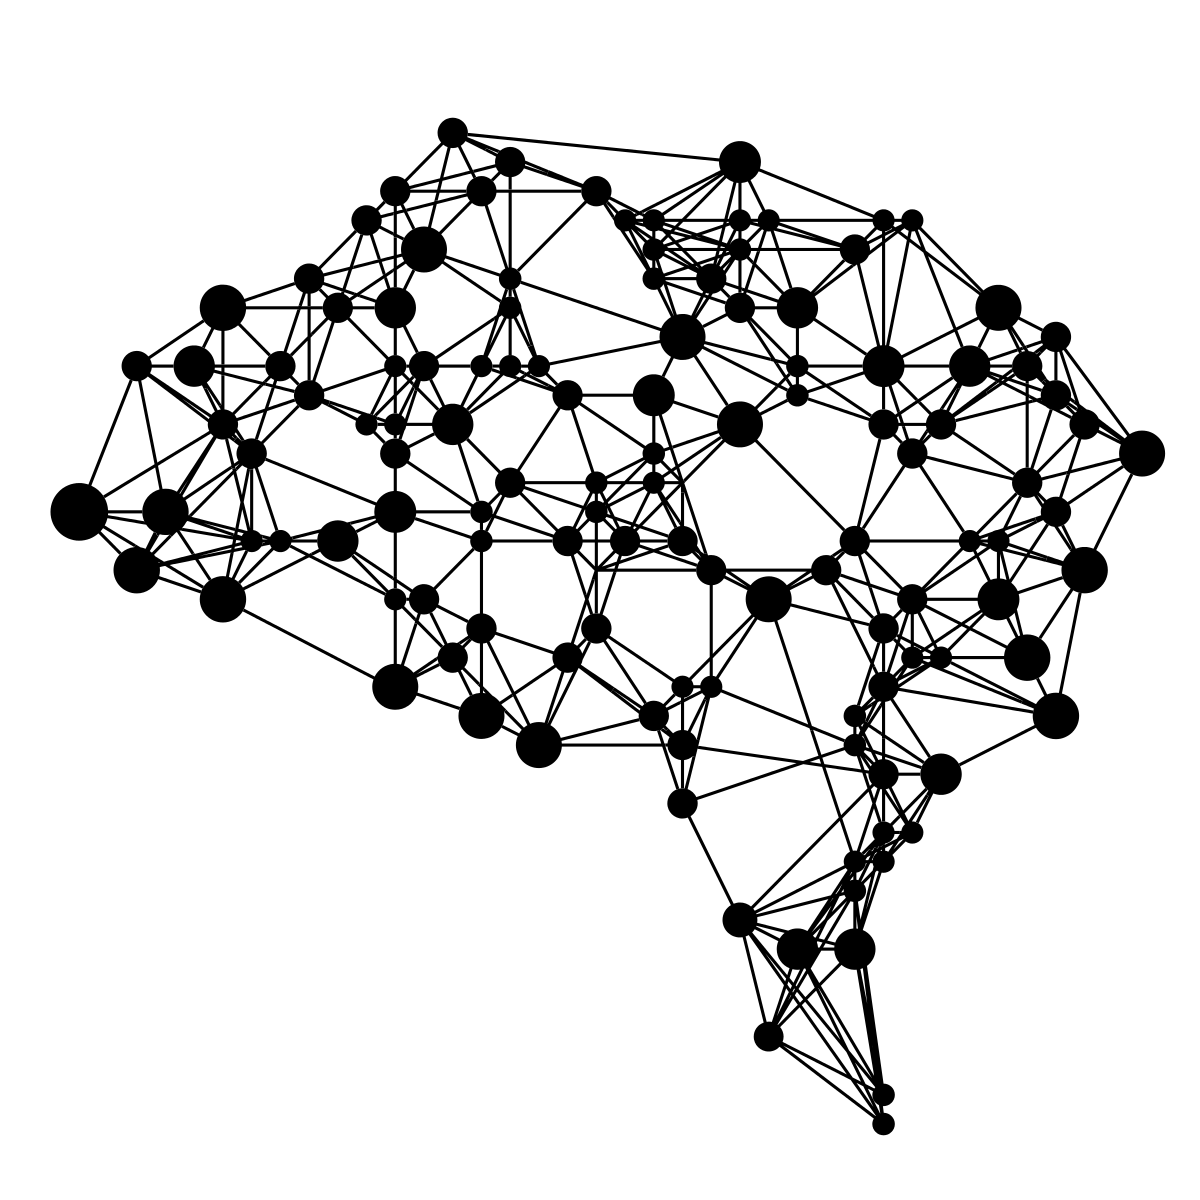
\includegraphics[totalheight=10cm]{titlepage.png}
    \cite{titlepageimage}
\end{center}

\newpage
\vspace*{\fill}
\input{lib/erklärung.tex}
\vspace*{\fill}

\newpage
\pagenumbering{arabic}
\tableofcontents

\newpage
\input{lib/einführung.tex}%TODO: Kapitel der App einfügen

\section{Neuronale Netzwerke}

\subsection{Geschichte}

Im Jahr 1943 wurde die erste Arbeit darüber geschrieben, wie Neuronen im Gehirn funktionieren könnten und die Autoren Warren McCulloch und Walter Pitts experimentierten sogar damit diese mit elektronischen Schaltkreisen nachzubauen.\footnote[6]{\cite[]{alogicalcalculus}} In den 1950er Jahren haben Forscher von IBM daran gearbeitet ein NN\footnote[7]{Kurzform für Neuronales Netzwerk, wird ab jetzt weiterhin verwendet.} mit einem Computer zu simulieren. Der Versuch scheiterte allerdings.\footnote[8]{\cite[Absatz 3]{nnhistory}} Immer wieder gab es kleinere Forschungsprojekte, ein sehr großer Durchbruch war aber 1975 die Entwicklung eines "`Backpropagation"' Algorithmus durch den Wissenschaftler Paul Werbos. Ähnliche Algorithmen wurden wiederholt und unabhängig entwickelt, aber Werbos' Algorithmus war der erste mit großer Bedeutung.\footnote[9]{\cite[]{paulwerbosbackpropagation}} Das Prinzip des Algorithmus wird auch heute noch verwendet, es ist dieser Algorithmus der dem Neuronalen Netzwerk das selbstständige Lernen ermöglicht.\footnote[10]{siehe Kapitel \ref{funktionsweise}}
\subsubsection{Zeitstrahl}

\begin{chronology}[10]{1940}{2020}{\textwidth}
    \event{1943}{Erste Arbeit und Experimente}
    \event[1950]{1960}{Bemühungen, ein NN digital umzusetzen}
    \event{1975}{Backpropagation Algorithmus}
\end{chronology}

\subsection{Aufbau}

\begin{center}
    \begin{tikzpicture}[x=1.5cm, y=1.5cm, >=stealth]

        \foreach \m/\l [count=\y] in {1,2,3,missing,4}
        \node [every neuron/.try, neuron \m/.try] (input-\m) at (0,2.5-\y) {};

        \foreach \m [count=\y] in {1,missing,2}
        \node [every neuron/.try, neuron \m/.try ] (hidden-\m) at (2,2-\y*1.25) {};

        \foreach \m [count=\y] in {1,missing,2}
        \node [every neuron/.try, neuron \m/.try ] (output-\m) at (4,1.5-\y) {};

        \foreach \l [count=\i] in {1,2,3,n}
        \draw [<-] (input-\i) -- ++(-1,0)
        node [above, midway] {$I_\l$};

        \foreach \l [count=\i] in {1,n}
        \node [above] at (hidden-\i.north) {$H_\l$};

        \foreach \l [count=\i] in {1,n}
        \draw [->] (output-\i) -- ++(1,0)
        node [above, midway] {$O_\l$};

        \foreach \i in {1,...,4}
        \foreach \j in {1,...,2}
        \draw [->] (input-\i) -- (hidden-\j);

        \foreach \i in {1,...,2}
        \foreach \j in {1,...,2}
        \draw [->] (hidden-\i) -- (output-\j);

        \foreach \l [count=\x from 0] in {Eingabe, Versteckte, Ausgangs}
        \node [align=center, above] at (\x*2,2) {\l \\ Ebene};

    \end{tikzpicture}
\end{center}

\subsection{Funktionsweise} \label{funktionsweise}

\subsubsection{Trainieren - Backpropagation}

\newpage
\printbibliography[heading=bibintoc, title={Literaturverzeichnis}]
\end{document}